%=============================================================
\chapter{研究動機}
\label{ch:motivation}
%=============================================================

% ─── 章節破題 ───────────────────────────────────────────────
大規模磁碟式圖 ANNS 的效能瓶頸，
表面上是「SSD 隨機讀取太慢」，
實際上是三層相互疊加的問題：
硬體佇列對並發 I/O 存在非線性懲罰、
演算法對「已收斂的搜尋」仍持續發出無效 I/O、
以及兩者在 server mode 的高並發環境下形成交叉放大效應。
本章從問題的根源逐層展開，
建立 PaceANN 設計的必要性基礎。

%-------------------------------------------------------------
\section{NVMe SSD 的非線性佇列延遲}
\label{sec:mot-ssd}
%-------------------------------------------------------------

NVMe SSD 的隨機讀取延遲並非固定常數，
而是佇列深度（queue depth）的函數。
圖~\ref{fig:fio-qd} 呈現以 \texttt{fio} 對本實驗 NVMe 裝置
進行 4\,KB 隨機讀取（\texttt{O\_DIRECT}，\texttt{libaio}）的量測結果。

\begin{figure}[htbp]
  \centering
  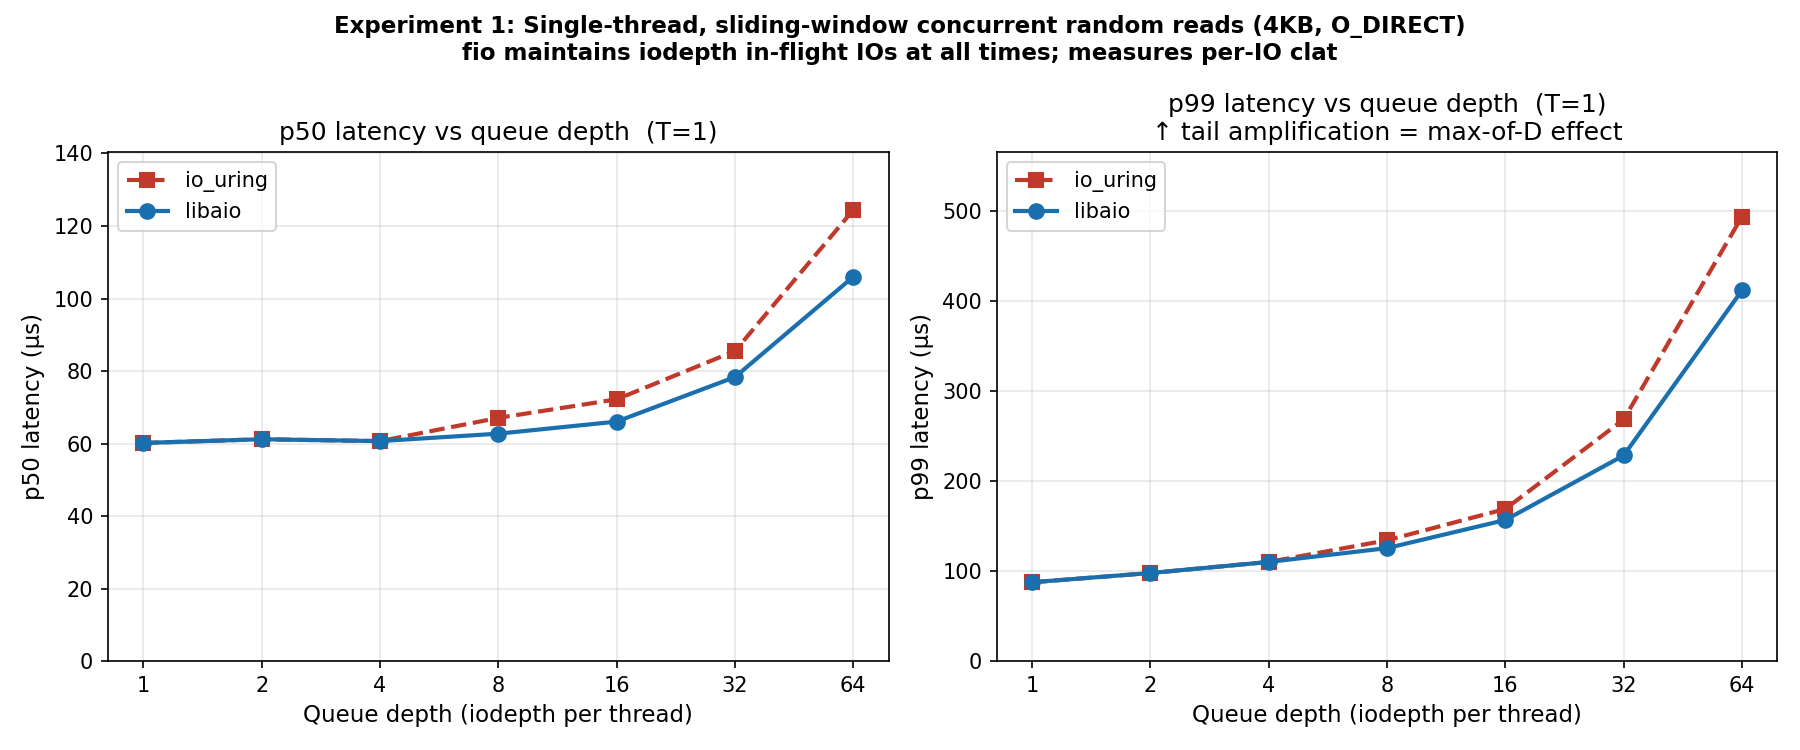
\includegraphics[width=0.72\textwidth]{figures/fio_queue_depth_latency.png}
  \caption{NVMe 裝置在不同佇列深度下的 4\,KB 隨機讀取延遲
  （\texttt{fio}，\texttt{O\_DIRECT}，\texttt{libaio}）。
  延遲隨佇列深度呈非線性增長，構成高並發下的尾延遲根源。}
  \label{fig:fio-qd}
\end{figure}

在低佇列深度（$D \leq 4$）時，裝置延遲穩定在 64--68\,$\mu$s；
這對應 NVMe controller 能夠立即服務、
幾乎不需要排隊的理想狀態。
隨著 $D$ 上升，延遲開始非線性增長：
$D = 32$ 時升至約 90\,$\mu$s，$D = 64$ 時達 131\,$\mu$s，
約為低佇列最佳點的 2.0 倍。

在 server mode 中這個問題更嚴峻。每個 worker thread 各自擁有獨立的 \texttt{io\_context\_t}，
並行地向同一顆 NVMe 裝置提交請求，系統層面的有效佇列深度是各線程提交量的總和
$D_{\text{eff}} = \sum_{t} D_t$。以排隊理論的 Little's Law（$L = \lambda W$）來看，
在服務率有限時，在制請求數增加會直接拉長每個請求的期望等待時間。
當 16 個 thread 各自維持 beam width 8 的並發展開時，最多會有約 128 個請求同時排在 NVMe 佇列裡，
遠超硬體的低延遲操作區間。也就是說，每一個不必要發出的 SSD 讀取，
都會延長系統中所有並發讀取的等待時間；在高並發的 server 環境下，這個代價由所有查詢共同承擔。

%-------------------------------------------------------------
\section{Beam Search 中的 I/O 邊際效益遞減現象}
\label{sec:mot-diminishing}
%-------------------------------------------------------------

DiskANN beam search 的資訊增益並非均勻分布在所有 hop 上。
直觀上，初期 hop 從 medoid 出發，
每次展開都能接觸到距離 query 明顯更近的節點，top-$k$ 快速收斂；
後期 hop 的探索空間已高度重疊，
展開新節點替換 top-$k$ 的概率急遽下降。

為了量化這個現象，我們做了一個 oracle early termination 分析：對 SIFT1M 的每筆查詢，
以完整預算（$L=150$，$W=8$）執行 beam search，並在每個 hop 結束後記下當下的 top-$k$；
再用 ground truth 找出最早達到最終 recall 的那個 hop，當作 oracle 停止點 $h^*$，
把 $L/W - h^*$ 視為無效 hop 數。結果呈現出一個結構性的問題（表~\ref{tab:oracle-summary}）。

\begin{table}[h]
\centering
\caption{Oracle ET 分析：不同 $L$ 設定下的 hop 效率
（SIFT1M，$W = 8$，$K = 10$）}
\label{tab:oracle-summary}
\begin{tabular}{rrrrrr}
\hline
$L$ & 平均實際 hop & Oracle 停止 hop & 無效 hop\,\% & 延遲節省上限\,\% & Recall \\
\hline
 20 &  6.9 & 6.2 & 10.2\% &  7.2\% & 0.9880 \\
 50 & 10.3 & 6.4 & 37.5\% & 36.9\% & 0.9977 \\
 80 & 13.5 & 6.5 & 52.3\% & 53.3\% & 0.9989 \\
100 & 16.2 & 6.5 & 60.0\% & 60.6\% & 0.9992 \\
150 & 22.2 & 6.5 & \textbf{70.7\%} & \textbf{71.2\%} & 0.9994 \\
\hline
\end{tabular}
\end{table}

以高 recall 所需的 $L = 150$ 為例，
平均每個 query 執行 22.2 個 hop，
但 oracle 只需 6.5 個 hop 就能達到相同 recall。
此後的 15.7 個 hop（70.7\%）純粹在收斂後繼續探索，
不帶來任何 recall 改善，
卻每個 hop 向 SSD 發出最多 $W = 8$ 個讀取請求。

固定 $L$ 的設計還有一個更根本的缺陷：它對異質的查詢難度系統性地誤配。
表~\ref{tab:oracle-cdf} 呈現 oracle 停止點的累積分布。

\begin{table}[h]
\centering
\caption{Oracle 停止 hop 的查詢累積分布（$L=150$，$W=8$）}
\label{tab:oracle-cdf}
\begin{tabular}{rc}
\hline
Oracle 停止 hop $h^* \leq h$ & 查詢累積比例 \\
\hline
$h \leq 4$ & 13.5\% \\
$h \leq 5$ & 64.8\% \\
$h \leq 6$ & 87.1\% \\
$h \leq 7$ & 94.0\% \\
$h \leq 11$ & 99.1\% \\
\hline
\end{tabular}
\end{table}

約 64.8\% 的查詢在第 5 個 hop 就完成收斂，卻被 $L=150$ 逼著跑到第 22 個 hop 才停，
每筆平均多做約 17 個無效 hop；這些查詢多半落在高密度聚集區，答案在局部鄰域裡很快就找得到。
另一方面，約 6\% 的查詢需要超過 7 個 hop 才收斂，它們位於資料分布的稀疏邊緣、或多個聚集區的交界，確實需要較大的 $L$ 保護。
固定 $L$ 的設計於是讓容易的查詢承擔了為困難查詢買保險的成本。

這個現象也不是 SIFT 資料集的特例。圖式索引（Vamana、HNSW）在建構時透過 robust pruning~\cite{subramanya2019diskann}
維持短路徑性質，讓 beam search 前幾個 hop 就能快速接近 query 的 Voronoi 鄰域；
一旦進入鄰域，後續 hop 探索的多半是鄰域內部的節點，對 top-$k$ 的邊際貢獻趨近於零。
這種收斂是 Vamana 式圖索引的固有特性，因此在任何採用類似圖結構的磁碟 ANNS 系統上，I/O 的邊際效益遞減都會存在。

%-------------------------------------------------------------
\section{無效 I/O 在並發 Server 環境的放大機制}
\label{sec:mot-tail}
%-------------------------------------------------------------

前兩節分別揭示了 SSD 的佇列非線性懲罰，
以及 beam search 中大量無效 hop 的存在。
兩者在 server mode 的高並發環境中形成交叉放大：
無效 hop 的 I/O 需求持續維持高 $D_\text{eff}$，
而高 $D_\text{eff}$ 使每個 SSD 讀取（包括有效 hop 的讀取）延遲上升，
進一步惡化尾延遲。

把這個問題量化一下。若系統有 $T$ 個 worker thread、各服務一個並發查詢，而每筆查詢的無效 hop 比例為 $\rho_w$（$L=150$ 時約 $0.71$），
那麼在有效佇列深度 $D_\text{eff} = T \cdot W_\text{bw}$ 之中，大約有 $\rho_w$ 比例的請求是可以被消除的浪費。
以 16 個 thread、beam width 8 估算，128 個並發 I/O 裡約有 91 個來自無效 hop；把它們消掉，有效佇列深度可從 128 降到約 37，
正好落在 SSD 延遲曲線（圖~\ref{fig:fio-qd}）明顯改善的區間。

尾延遲（P99/P999）在 server mode 下比平均值更脆弱，這來自兩個交疊的效應。
一方面，佇列競爭本身帶有隨機性：各 thread 的 hop 並不同步，少數查詢的 SSD 讀取剛好集中在壅塞高峰，等待時間遠超平均，形成長尾。
另一方面，等待效應會串聯：一筆查詢的有效 hop 若被背景的無效 I/O 拖慢而延後完成，對應的 thread 就無法及時服務後面排隊的查詢，延遲因此往後傳播。
這兩點讓 P99 對 $D_\text{eff}$ 的敏感度高於平均延遲，在高並發下表現為 P99/mean 比值的急劇上升。
因此，有效管理 $D_\text{eff}$ 是改善 P99 的必要條件，而不只是一個加速手段。

現有方法多半沒有從這個角度切入。Starling~\cite{wang2024starling} 以 page grouping 提升每次 I/O 的資訊密度，讓較少的 hop 就能達到相同 recall，
但它改善的是每個 hop 的 I/O 效率，並不偵測、也不終止收斂後的無效 hop，$\rho_w$ 的問題依舊存在。
PipeANN~\cite{osdi25pipeann} 以 pipelined async I/O 重疊計算與 I/O 來隱藏部分延遲，但總 I/O 量沒有減少，佇列一旦飽和效益就有限。
這些方法都在優化「每個 I/O 的成本」，而真正的問題其實是「不必要的 I/O 根本不該被發出」。

%-------------------------------------------------------------
\section{核心洞察：收斂可在零 I/O 代價下偵測}
\label{sec:mot-insight}
%-------------------------------------------------------------

上述分析的出口，在於能否在搜尋過程中即時判斷某筆查詢的 top-$k$ 是否已收斂，而且這個判斷本身不能再引入額外的 SSD I/O，否則就成了新的負擔。

關鍵在於，判斷收斂所需的資訊其實都已經在 DRAM 裡。DiskANN 在記憶體中保有所有節點的 PQ 壓縮碼，用來在 beam search 中對尚未讀取鄰居的候選快速排序；
計算一個 PQ 近似距離只是純 CPU 操作，約 10\,ns，比 SSD 讀取的百微秒快了四個數量級。同時，那些已經展開、讀回全精度向量的候選，可以直接算出精確距離。
於是在每個 hop 之前，我們可以拿 frontier 中最有希望（PQ 下界最小）的未展開候選，去和目前已收斂候選的精確距離相比：
如果連前者這個樂觀估計都已明顯劣於後者，繼續展開幾乎不可能再換掉任何 top-$k$ 節點，就可以停下。
整個判斷都在 DRAM 中以 $O(1)$ 的 CPU 操作完成，不讀取任何 SSD 資料。第~\ref{ch:arch}~章會把這個條件正式化為跨尺度的精確門檻。

PQ 距離只是近似值，會系統性地低估真實距離（量化誤差）。這代表即使停止條件成立，繼續展開偶爾仍可能改善 recall，
因此判斷用的門檻 $\theta$ 需要留一點餘裕：$\theta$ 越接近 1 越保守，假陽性少但省下的 hop 也少；$\theta$ 越大越積極，省得多但 recall 代價高。
如何在不同資料集與 recall 要求下選出合適的 $\theta$，是第~\ref{ch:method}~章要處理的問題之一。

這個判斷還有一個前提：拿來當基準的已收斂結果必須夠穩定。若此刻 top-$k$ 才剛開始累積、覆蓋不足，
用來比較的距離就不可靠，容易造成假陽性而提早停止。這種情況在搜尋最初期（前幾個 hop）最難避免，因為 beam search 才剛從 medoid 出發、候選還很少。
把高頻節點留在快取正好能緩解這點：若前幾個 hop 以 DRAM 而非 SSD 的速度完成，top-$k$ 能在更短的時間內建立足夠覆蓋，
後續的停止判斷也就更可靠。這也是為什麼快取與早停是彼此需要的協同設計，而不是兩個各自獨立的最佳化剛好湊在一起。

%-------------------------------------------------------------
\section{研究問題的形式化}
\label{sec:mot-rq}
%-------------------------------------------------------------

基於上述動機分析，本研究瞄準下列核心問題：

\begin{description}
  \item[\textbf{RQ1.}] 能否設計一個基於 PQ 距離的收斂偵測條件，
    使 beam search 能夠對每個 query 自適應地停止於
    \emph{個別}收斂點，而非全局固定的 $L$？

  \item[\textbf{RQ2.}] 如何設計 DRAM 快取策略，
    使搜尋初期的 top-$k$ 覆蓋足夠穩定，
    從而讓收斂偵測條件在高 recall 要求下保持可靠？

  \item[\textbf{RQ3.}] 上述機制在 server mode 的高並發下，
    能否有效降低 $D_\text{eff}$ 並改善 P99 尾延遲，
    同時維持與 Starling 等 SOTA 系統的競爭力？

  \item[\textbf{RQ4.}] 收斂偵測的閾值 $\theta$ 對不同資料集分布的敏感度
    如何量化，設計者應如何選擇？
\end{description}

這四個問題分別對應本論文的架構設計（第~\ref{ch:arch}~章）、
參數分析（第~\ref{ch:method}~章）以及實驗評估（第~\ref{ch:evaluation}~章）。
